\begin{figure}
  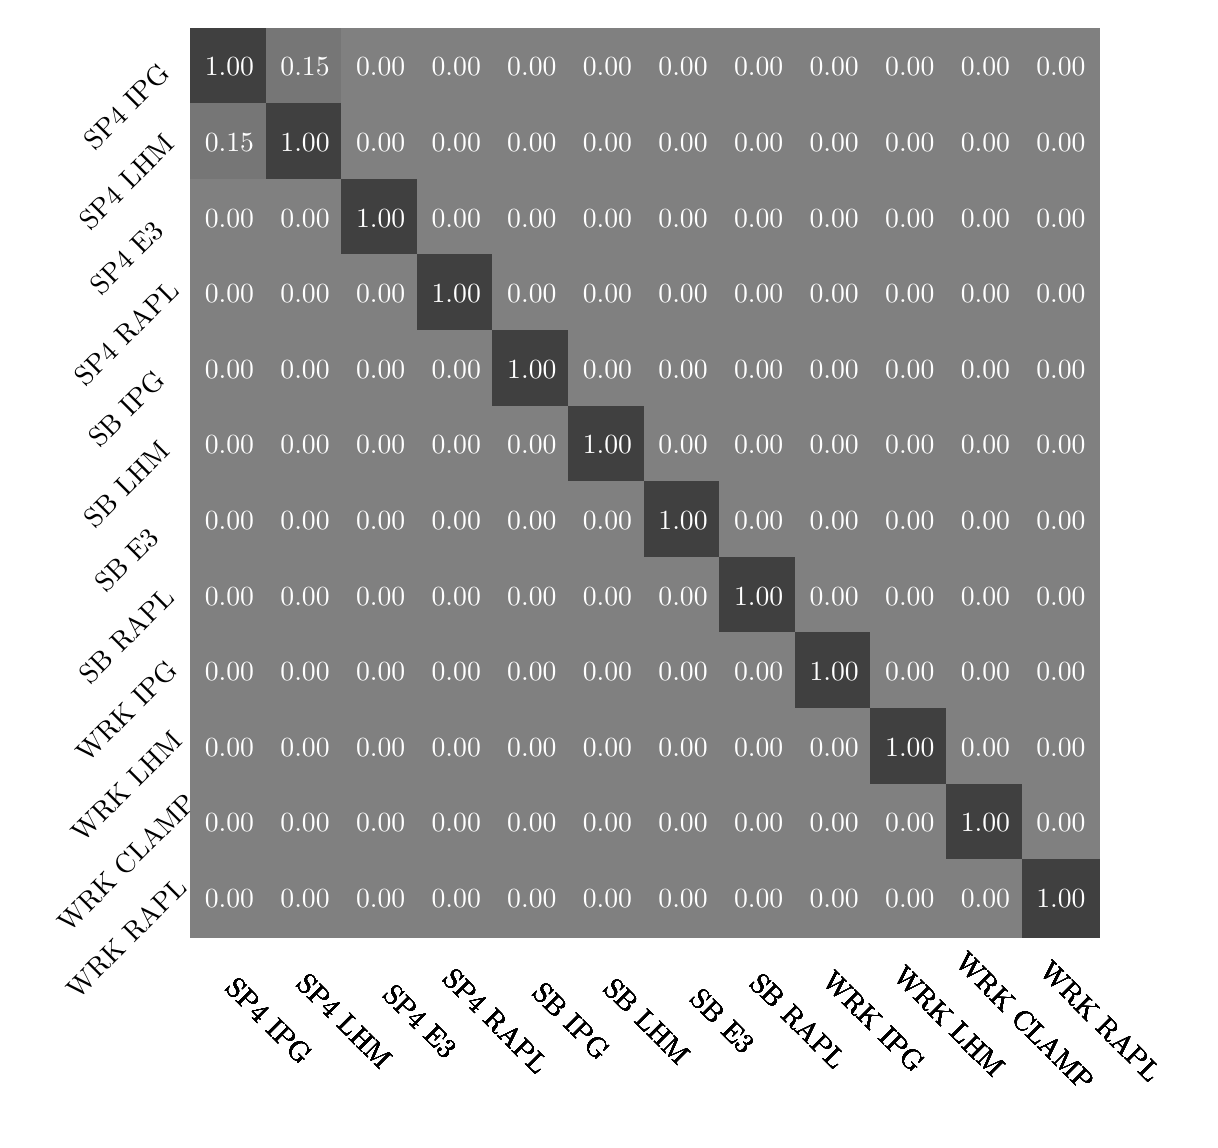
\begin{tikzpicture}[scale=0.6]
    \foreach \y [count=\n] in {{1.00, 0.15, 0.00, 0.00, 0.00, 0.00, 0.00, 0.00, 0.00, 0.00, 0.00, 0.00},{0.15, 1.00, 0.00, 0.00, 0.00, 0.00, 0.00, 0.00, 0.00, 0.00, 0.00, 0.00},{0.00, 0.00, 1.00, 0.00, 0.00, 0.00, 0.00, 0.00, 0.00, 0.00, 0.00, 0.00},{0.00, 0.00, 0.00, 1.00, 0.00, 0.00, 0.00, 0.00, 0.00, 0.00, 0.00, 0.00},{0.00, 0.00, 0.00, 0.00, 1.00, 0.00, 0.00, 0.00, 0.00, 0.00, 0.00, 0.00},{0.00, 0.00, 0.00, 0.00, 0.00, 1.00, 0.00, 0.00, 0.00, 0.00, 0.00, 0.00},{0.00, 0.00, 0.00, 0.00, 0.00, 0.00, 1.00, 0.00, 0.00, 0.00, 0.00, 0.00},{0.00, 0.00, 0.00, 0.00, 0.00, 0.00, 0.00, 1.00, 0.00, 0.00, 0.00, 0.00},{0.00, 0.00, 0.00, 0.00, 0.00, 0.00, 0.00, 0.00, 1.00, 0.00, 0.00, 0.00},{0.00, 0.00, 0.00, 0.00, 0.00, 0.00, 0.00, 0.00, 0.00, 1.00, 0.00, 0.00},{0.00, 0.00, 0.00, 0.00, 0.00, 0.00, 0.00, 0.00, 0.00, 0.00, 1.00, 0.00},{0.00, 0.00, 0.00, 0.00, 0.00, 0.00, 0.00, 0.00, 0.00, 0.00, 0.00, 1.00},} {
    % column labels
    \foreach \a [count=\n] in {SP4 IPG,SP4 LHM,SP4 E3,SP4 RAPL,SB IPG,SB LHM,SB E3,SB RAPL,WRK IPG,WRK LHM,WRK CLAMP,WRK RAPL} {
      \node[minimum size=10mm, xshift=0.5cm, rotate=-45] at (\n*1.6, -21.8) {\a};
    }
    % heatmap tiles
    \foreach \x [count=\m] in \y {
      \pgfmathsetmacro{\xa }{(\x + 1) / 2 * 100}
      \node[fill=darkgray!\xa!lightgray, minimum size=10mm, text=white, font={\normalsize}] at (\m*1.6,-\n*1.6) {\x};
    }
  }
    % row labels
    \foreach \a [count=\i] in {SP4 IPG,SP4 LHM,SP4 E3,SP4 RAPL,SB IPG,SB LHM,SB E3,SB RAPL,WRK IPG,WRK LHM,WRK CLAMP,WRK RAPL} {
      \node[minimum size=10mm, xshift=-0.35cm, yshift=-0.5cm, rotate=45] at (0,-\i*1.6) {\a};
    }
  \end{tikzpicture}
  \caption{Here the results for the FannkuchRedux can be seen}
  \label{tab:HeatFannkuchRedux}
  \end{figure}